\section{Gaussian importance sampling for state space models}
\label{sec:gaussian_importance_sampling_for_state_space_models}

% two types of proposals: direct, SSMs
For the types of models considered in this thesis, importance sampling is used to infer the posterior distribution. Given a state space model of the form \eqref{def:ssm} and observations $Y = Y_{:n}$, let $\P$ be the distribution of the states $X=X_{:n}$, conditional on $Y$ and $f$ be a function of interest. The task at hand is now to find a suitable proposal $\G$, using the methods presented in the last section. If $n$ is large, the posterior distribution lives in a high dimensional state of dimension $m\cdot n$ so to obtain $\G$ efficiently, we should exploit the available structure. Additionally, we want $\G$ to be tractable, so simulating from it is possible and evaluating the weights $w$ up to a constant is possible. 

The multivariate Gaussian distribution is a good candidate in this setting, as simulating from it is straightforward and its density can be evaluated analytically. However, naively performing the optimal importance sampling methods from the previous section for all multivariate Gaussians is computationally inefficient as the family of distributions has $\mathcal O((n\cdot m)^{2})$ many parameters. We can, however, exploit the available structure of the \gls{ssm} to find parameterizations with fewer parameters by either using smoothing distributions of \glspl{glssm} (\Cref{subsec:glssm-approach}) or approximating with a Gaussian discrete-time Markov process (\Cref{subsec:markov-approach}). 

% discuss if there actually is a Gaussian close to the target, see heavy tails etc.
Using Gaussian proposals, while computationally efficient, also comes with some drawbacks. The whole procedure hinges on the assumption that there is a Gaussian that is, close to the target distribution. In the setting of \glspl{ssm} this is not guaranteed, as the targets may contain multiple modes or heavy tails, features that may, in the worst case, lead to inconsistent importance sampling estimates. At least for the models considered in \Cref{cha:analysis_of_selected_models}, the targets arise as posterior distributions of \gls{lcssm} and as such they are unimodal and have non-heavy tails, i.e. there is a Gaussian distribution such that importance sampling is feasible \todo{rethink, is this really the case, for LCSSM it depends on log-partition function of observations}. 
Additionally, even if there is a Gaussian distribution that facilitates consistent importance sampling, finding it in practice may be complicated, as the proposals generated by the \gls{la}, \gls{cem} and \gls{eis} have deteriorating performance for fixed sample size $N$ (in terms of \gls{ess} and convergence) with increasing dimension \todo{ref to chapter, check that I also present that there}.

\todo{small lit. review}
% first: Gaussian SSMs
\subsection{\texorpdfstring{The \gls{glssm}-approach}{The GLSSM-approach}}
\label{subsec:glssm-approach}
The first approach \todo{cite} is motivated by the fact that the target posterior is again a Markov process, as are posteriors in \glspl{glssm}. Additionally, the posterior distribution in \gls{glssm}s is again Gaussian, and straightforward to simulate from by, e.g., the FFBS \todo{cite} algorithm. Thus parameterizing the proposals $\G$ by the posterior of a suitably chosen \gls{glssm} may be a fruitful approach.
For the models we consider in this thesis, the distribution of states is already Gaussian and the observations are conditionally independent given the states. Thus a natural \gls{glssm} to use as a proposal consists of keeping the prior distribution of states and replacing the distribution of observations with conditionally independent Gaussian distributions and the actual observations by synthetic ones. By the assumed conditional independence, this model only needs $2 p\cdot (n + 1)$ many parameters, $p\cdot (n + 1)$ for the synthetic observations and $p\cdot (n + 1)$ for their variances. We term this approach the \textbf{\gls{glssm}-approach} to importance sampling.

In total, the \gls{glssm}-approach considers parametric proposals $\G_{\psi}$ of the form
\begin{align}
    \begin{split}
    \label{eq:glssm-proposal}
    \G_{\psi} &= \mathcal L(X | Z = z),\\
    Z_{t} &= B_{t} X_{t} + \eta_{t},\\
    \eta_{t} &\sim \mathcal N \left( 0, \Omega_{t} \right),\\
    \Omega_{t} &= \diag \left( \omega^{2}_{t} \right) = \diag \left( \omega^{2}_{t,1}, \dots, \omega^{2}_{1,p} \right).
    \end{split}
\end{align}
where the distribution of $X$ is given by \eqref{eq:glssm_states}, $\psi = \left( z, \omega^{2} \right)$ for $z = \left( z_{0}, \dots, z_{n} \right) \in \R^{n \times m}$ and $\omega^{2} = \left( \omega^{2}_{0}, \dots, \omega^{2}_{n} \right) \in \R^{n \times m}$. Alternatively the natural parametrization $\psi = \left( z \oslash \omega^{2}, - 1 \oslash \left( 2 \omega^{2} \right) \right)$ may also be used, where $\oslash$ is the Hadamard, i.e. entry-wise, division. Simulation from $\G_{\psi}$ may be efficiently implemented by the FFBS algorithm, as $\G_{\psi}$ is the smoothing distribution of a \gls{glssm}. 

% weights
In this setting, the importance sampling weights are given by 
$$
w(x) = \frac{p(x|y)}{g(x|z)} = \frac{p(y|x)p(x)}{g(z|x)p(x)} \frac{g(z)}{p(y)} \propto \prod_{t = 0}^n \frac{p(y_{t}|x_{t})}{g(z_{t}|x_{t})},
$$
% Signals
so they can be computed efficiently. Additionally, as \todo{add signal restriction above} $p(y_{t}|x_{t})$ and $g(z_{t}|x_{t})$ depend on $x_{t}$ only through the signal $s_{t} = B_{t}x_{t}$, we have 
$$
w(x) \propto \prod_{t = 0}^{n}\frac{p(y_{t}|s_{t})}{g(z_{t}|s_{t})},
$$
which implies that auto-normalized weights may be calculated by using the signal smoother \cite[Theorem 2]{Jungbacker2007Monte}.
\todo{introduce LCSSM with linear signals above}
As \citeauthor{Durbin2012Time} \cite[Section 4.5.3]{Durbin2012Time} argue, it is often computationally more efficient to treat only on the signals $\left(S_{t}\right)_{t=0,\dots,n}$ instead of the states $ \left( X_{t}  \right)_{t = 0, \dots, n}$, the idea being that the dimension of $S_{t}$, $p$, is usually much smaller than that of $X_{t}$, $m$. 

% sample from states still possbile if doingo nly signals, weights don't change
As the joint distribution of $(X, S)$ is a Gaussian distribution, by \Cref{lem:gaussian_conditional} $X|S = s$ is again Gaussian \todo{add degernate case to gaussian conditional lemma}, with known conditional mean and covariance matrix and density $p(x|s) = g(x|s)$. If $(\tilde X_{t})_{t=0,\dots,n}$ is a draw from this conditional distribution a quick calculation reveals that a.s. $B_{t} \tilde X_{t} = S_{t}$, and so, as expected, the weights $w(\tilde X_{t})$ are a.s. constant and given by (up to the integration constant) $\prod_{t = 0}^{n}\frac{p(y_{t}|s_{t})}{g(y_{t}|s_{t})}$. Producing a draw from this conditional distribution can be achieved by the FFBS algorithm (\Cref{alg:ffbs}), as $(X, S)$ form a \gls{glssm} with degenerate observation covariance matrices $\Omega_{t} = 0$.

By the assumed conditional independence of observations given signals, we have
$$
p(x, s|y) \propto p(x|s) p(s|y),
$$
and so if one is interested in the states, rather than the signals, importance sampling with the proposal \Cref{eq:glssm-proposal} can be achieved in a two-step procedure: first sample from $g(s|z)$, then run the FFBS algorithm to sample from $g(x|s) = p(x|s)$ using the same weights for MC-integration. 

% degenerate distribution, exponential family of proposals for signals
The \gls{glssm}-approach is the standard approach for finding the \gls{la} in \gls{lcssm} \cite{Durbin1997Monte,Durbin2012Time} and may even be applied when the observation densities are not log-concave\cite{Jungbacker2007Monte}. The approach also leads to efficient implementation for \gls{eis} \cite{Koopman2019Modified}. However, as will become apparent in the later part of this section, it is infeasible for the \gls{cem} if $n$ is large. 


We now give a concise overview over how to perform the \gls{la} and \gls{eis} for \gls{lcssm}, but refer the reader for more details to the respective literature.
The \gls{la} \todo{...}

\begin{algorithm}
    \caption{The \gls{la} for \gls{lcssm}}
    \label{alg:la}
\end{algorithm}

\begin{algorithm}
    \caption{\gls{eis} for \gls{lcssm}}
    \label{alg:eis}
\end{algorithm}
% SSMs may utilize KF/KS to perform importance sampling
% LA: cite Koopman paper
% EIS: cite papers, MEIS NEIS


% CE: two variants 
%% GLSSM approach fails: 
For the \gls{cem}, using the \gls{glssm}-approach turns out to be difficult numerically. For a high-level argument of why this is true, let us ignore the Markov structure of the model for the moment. As the \gls{cem} matches moments of the target and proposal, applying it to fit model \eqref{eq:glssm-proposal} amounts to matching the moments of $\G_{\psi}$ to those of the target posterior $\mathcal L (X | Y = y)$ in the \gls{ssm}. Unfortunately, the covariance of $\G_{\psi}$ is given by $ \left( \Sigma^{-1} + B^{T}\Omega^{-1} B \right)^{-1}$, where $\Sigma$ is the covariance of all states, $B = \bdiag (B_{0}, \dots, B_{n})$ and $\Omega = \bdiag \left( \Omega_{0}, \dots, \Omega_{n} \right)$. Choosing the diagonal matrix $\Omega$ such that the covariance of $\G_{\psi}$ matches this expression is numerically expensive: we either need to invert the large (dimension $(n + 1)m \times (n + 1)m$) covariance matrix, or solve numerically for the $(n + 1)p$ parameters. The problem at hand is that we cannot decouple this into $(n + 1)$ equations of dimension $p$ as we did for \gls{eis}, because all entries of $(\Sigma^{-1} + B^{T}\Omega^{-1} B)^{-1}$ depend on all entries of $\Omega$. 

To make matters more concrete, the \gls{cem} finds $\psi = (z, \omega^{2})$ such that model \eqref{eq:glssm-proposal} maximizes the cross entropy with the target $\P^{X|Y=y}$. For simplicity, let us assume that $m = p$, $B$ is the identity and we only observe a single $y$. Using \Cref{lem:gaussian_conditional}, we see that when $X\sim\mathcal N(\mu, \Sigma)$, the conditional distribution of $X$ given $Z=z$, $\G_{\psi}$, is a Gaussian distribution with mean $\tilde \mu =  \mu + \Sigma \left( \Sigma  + \Omega \right)^{-1} \left( z - \mu \right)$  and covariance matrix $\tilde\Sigma = \left( \Sigma ^{-1} + \Omega^{-1}\right)^{-1}$ for $\Omega = \diag \left( \omega^{2} \right)$, where $\omega^{2} > 0$. Assuming that $\Sigma$ is non-singular, we can reparameterize the objective function of the \gls{cem} by $\tilde \mu$,
\begin{align}
    \label{eq:cem_reparametrization}
    \begin{split}
    \max_{z, \omega^{2}} \int p(x|y) \log g_{\psi}(x|z) \mathrm dx &= \max_{\tilde\mu, \omega^{2}} \int p(x|y) \left( - \frac{1}{2} (x - \tilde \mu)^{T} \tilde \Sigma ^{-1} \left( x - \tilde \mu \right)  - \frac{1}{2} \log\det \tilde \Sigma \right)  \d x\\
&= \max_{\tilde \mu, \omega^{2}} - \frac{1}{2} (\gamma - \tilde \mu)^{T}\tilde \Sigma ^{-1} ( \gamma - \tilde \mu) - \frac{1}{2} \operatorname{trace} \left( \tilde \Sigma^{-1} \Gamma \right) - \frac{1}{2} \log\det\tilde\Sigma,
    \end{split}
\end{align}
where $\gamma = \E \left( X | Y = y \right)$ and $\Gamma = \cov \left( X | Y = y \right)$. 
Thus the optimal $\tilde \mu$ is $\gamma$ and to find $\omega^{2}$ we have to minimize 
$$
\operatorname{trace} \left( \left( \Sigma^{-1} + \Omega^{-1} \right) \Gamma \right) - \log\det \left( \Sigma^{-1} + \Omega^{-1} \right).
$$
Taking the derivative w.r.t. $\frac{1}{\omega^{2}}$, we see that 
\begin{align}
\label{eq:gamma_post}
\Gamma_{i,i} = \left(\left( \Sigma^{-1} + \diag \left( \frac{1}{\omega_{1}}, \dots, \frac{1}{\omega_{p}}\right) \right)^{-1}\right)_{i,i} = \left( \Sigma - \Sigma \left( \Sigma + \Omega \right)^{-1}\Sigma \right)_{i,i} %= \Sigma_{i,i} - \Sigma_{i}^T \left( \Sigma + \Omega \right)^{-1} \Sigma_{i},
\end{align}
has to hold for all $i = 1, \dots, p$, i.e. we have to choose $\omega^{2}$ such that the posterior marginal variances $\Gamma_{i,i}$ coincide with the marginal variances of $\G_{\psi}$.

Several problems arise: First of all, \Cref{eq:gamma_post} is not guaranteed to have a solution. For the $i$-th unit-vector $e_{i}\in\R^{p}$ we can reformulate \Cref{eq:gamma_post} to 
$$
\Sigma_{i,i} - \Gamma_{i,i} = e_{i}^T\Sigma^{T} \left( \Sigma + \Omega \right)^{-1}\Sigma e_{i} > 0
$$
and so we require $\Gamma_{i,i} < \Sigma_{i,i}$. While the law of total covariance asserts that
$$
\Sigma = \E \underbrace{\cov \left( X | Y \right)}_{=\Gamma} + \cov \left( \E \left( X | Y \right) \right),
$$
it does not guarantee $\Gamma \prec \Sigma$, which would imply $\Gamma_{i,i} < \Sigma_{i,i}$. 
\todo{can we find example?}

Second, even if there is an analytical solution $\Omega$ to \Cref{eq:gamma_post}, in the \gls{cem} we replace $\Gamma_{i,i}$ by the observed marginal variances $\hat\Gamma_{i,i}$ obtained by importance sampling. The variation introduced by simulation can then lead to situations where $\hat\Gamma_{i,i} > \Sigma_{i,i}$. As an example take $X \sim \mathcal N(0, 1)$, and $Y = X + \eta$ for $\eta \sim \mathcal N(0, \omega^{2})$. Then the conditional variance of $X$ given $Y = y$ is $\Gamma = 1 - \frac{1}{1 + \omega^{2}}$. Given $N$ i.i.d. samples $X^{1}, \dots X^{N}$ from this distribution, their empirical variance $\hat \Gamma = \frac{1}{N} \sum_{i = 1}^{N} (X^{i} - \bar X)^{2} $ follows a scaled $\chi_{N - 1}^{2}$ distribution, i.e. $ \frac{N\hat\Gamma}{\Gamma} \sim \chi^{2}_{N - 1}$. Notice that we use the non-Bessel corrected version of the empirical variance here, as it is the maximum-likelihood estimate. 

Then $$\P \left( \hat \Gamma > 1 \right) = \P \left( \frac{N \hat \Gamma}{\Gamma} > \frac{N}{\Gamma} \right) = 1 - F_{\chi^{2}_{N-1}} \left( N \left( 1 + \frac{1}{\omega^{2}} \right) \right)$$ is the probability that \Cref{eq:gamma_post} has no solution $\omega^{2} \in \R_{\geq 0}$ \todo{introduce symbol}. Here $F_{\chi^{2}_{N - 1}}$ is the cumulative distribution function of the $\chi^{2}_{N - 1}$ distribution. As $\omega^{2}$ goes to $\infty$, this probability approaches $1 - F_{\chi^{2}_{N - 1}}(N)$ which, for large $N$, is approximately $1 - F_{\chi^{2}_{N - 1}} (N - 1) \approx \frac{1}{2}$, as $\chi^{2}_{N-1} \approx \mathcal N\left(N - 1, 2 (N-1)\right)$ \cite[Section 18.5]{Johnson1994Continuous}.
We illustrate this in \Cref{fig:ce_prob_failure}, displaying the probability of failure in this setting for various combinations of $N$ and $\omega^{2}$. In this figure, we see that with growing $N$ the threshold for $\omega^{2}$ leading to non-negligible failure probability becomes larger, as expected. 
Thus, even in the very simple univariate Gaussian setting, for every $N$ there is an $\omega^{2}$ such that the \gls{cem} fails for \Cref{eq:glssm-proposal} with practically relevant probability. 

\begin{figure}
    \resizebox{\textwidth}{!}{%
        % Created by tikzDevice version 0.12.6 on 2024-07-02 14:22:08
% !TEX encoding = UTF-8 Unicode
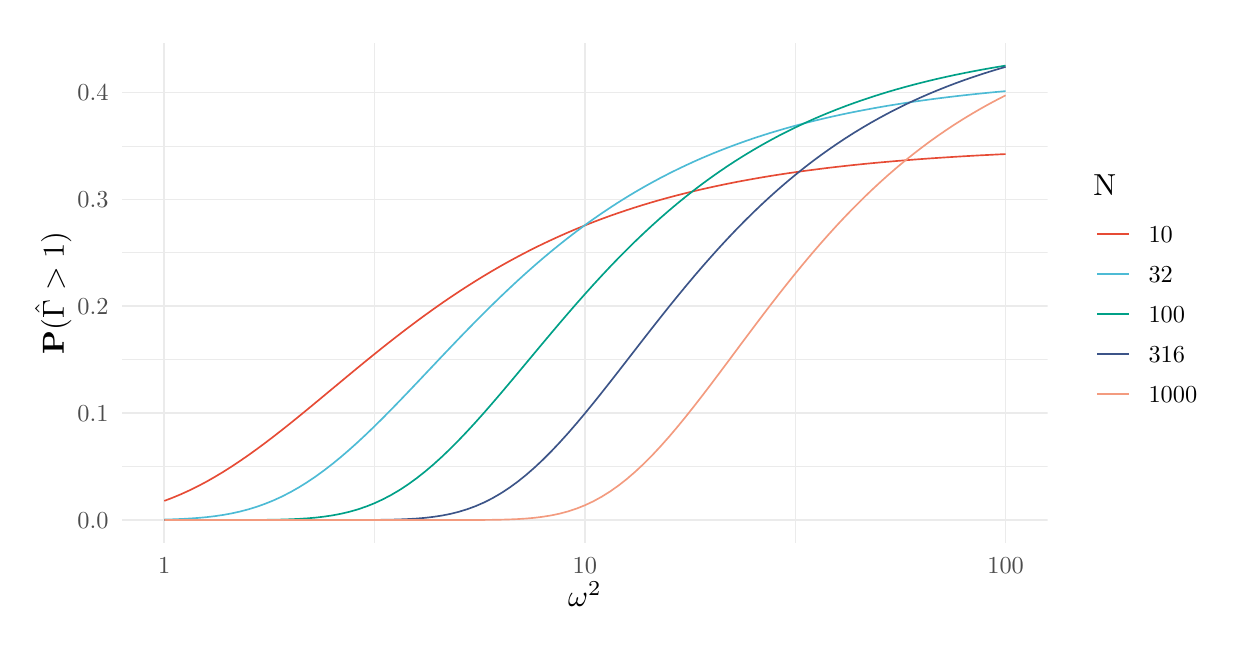
\begin{tikzpicture}[x=1pt,y=1pt]
\definecolor{fillColor}{RGB}{255,255,255}
\path[use as bounding box,fill=fillColor,fill opacity=0.00] (0,0) rectangle (433.62,216.81);
\begin{scope}
\path[clip] ( 34.16, 30.69) rectangle (368.57,211.31);
\definecolor{drawColor}{gray}{0.92}

\path[draw=drawColor,line width= 0.3pt,line join=round] ( 34.16, 58.20) --
	(368.57, 58.20);

\path[draw=drawColor,line width= 0.3pt,line join=round] ( 34.16, 96.82) --
	(368.57, 96.82);

\path[draw=drawColor,line width= 0.3pt,line join=round] ( 34.16,135.43) --
	(368.57,135.43);

\path[draw=drawColor,line width= 0.3pt,line join=round] ( 34.16,174.05) --
	(368.57,174.05);

\path[draw=drawColor,line width= 0.3pt,line join=round] (125.36, 30.69) --
	(125.36,211.31);

\path[draw=drawColor,line width= 0.3pt,line join=round] (277.37, 30.69) --
	(277.37,211.31);

\path[draw=drawColor,line width= 0.6pt,line join=round] ( 34.16, 38.90) --
	(368.57, 38.90);

\path[draw=drawColor,line width= 0.6pt,line join=round] ( 34.16, 77.51) --
	(368.57, 77.51);

\path[draw=drawColor,line width= 0.6pt,line join=round] ( 34.16,116.13) --
	(368.57,116.13);

\path[draw=drawColor,line width= 0.6pt,line join=round] ( 34.16,154.74) --
	(368.57,154.74);

\path[draw=drawColor,line width= 0.6pt,line join=round] ( 34.16,193.35) --
	(368.57,193.35);

\path[draw=drawColor,line width= 0.6pt,line join=round] ( 49.36, 30.69) --
	( 49.36,211.31);

\path[draw=drawColor,line width= 0.6pt,line join=round] (201.36, 30.69) --
	(201.36,211.31);

\path[draw=drawColor,line width= 0.6pt,line join=round] (353.37, 30.69) --
	(353.37,211.31);
\definecolor{drawColor}{RGB}{230,75,53}

\path[draw=drawColor,line width= 0.6pt,line join=round] ( 49.36, 45.81) --
	( 52.40, 46.97) --
	( 55.44, 48.24) --
	( 58.48, 49.62) --
	( 61.52, 51.12) --
	( 64.56, 52.73) --
	( 67.60, 54.46) --
	( 70.64, 56.28) --
	( 73.68, 58.21) --
	( 76.72, 60.23) --
	( 79.76, 62.33) --
	( 82.80, 64.52) --
	( 85.84, 66.77) --
	( 88.88, 69.09) --
	( 91.92, 71.46) --
	( 94.96, 73.88) --
	( 98.00, 76.34) --
	(101.04, 78.83) --
	(104.08, 81.34) --
	(107.12, 83.86) --
	(110.16, 86.39) --
	(113.20, 88.92) --
	(116.24, 91.44) --
	(119.28, 93.95) --
	(122.32, 96.44) --
	(125.36, 98.90) --
	(128.40,101.34) --
	(131.44,103.74) --
	(134.48,106.10) --
	(137.52,108.43) --
	(140.56,110.71) --
	(143.60,112.94) --
	(146.64,115.12) --
	(149.68,117.26) --
	(152.72,119.34) --
	(155.76,121.37) --
	(158.80,123.34) --
	(161.84,125.26) --
	(164.88,127.13) --
	(167.92,128.94) --
	(170.96,130.70) --
	(174.00,132.40) --
	(177.04,134.04) --
	(180.08,135.64) --
	(183.12,137.18) --
	(186.16,138.67) --
	(189.20,140.10) --
	(192.24,141.49) --
	(195.28,142.83) --
	(198.32,144.12) --
	(201.36,145.36) --
	(204.40,146.56) --
	(207.44,147.71) --
	(210.48,148.82) --
	(213.52,149.88) --
	(216.56,150.91) --
	(219.60,151.89) --
	(222.64,152.84) --
	(225.68,153.75) --
	(228.72,154.62) --
	(231.76,155.46) --
	(234.80,156.26) --
	(237.84,157.03) --
	(240.88,157.77) --
	(243.92,158.48) --
	(246.97,159.16) --
	(250.01,159.81) --
	(253.05,160.44) --
	(256.09,161.04) --
	(259.13,161.61) --
	(262.17,162.16) --
	(265.21,162.69) --
	(268.25,163.20) --
	(271.29,163.68) --
	(274.33,164.14) --
	(277.37,164.58) --
	(280.41,165.01) --
	(283.45,165.41) --
	(286.49,165.80) --
	(289.53,166.18) --
	(292.57,166.53) --
	(295.61,166.87) --
	(298.65,167.20) --
	(301.69,167.51) --
	(304.73,167.81) --
	(307.77,168.09) --
	(310.81,168.36) --
	(313.85,168.62) --
	(316.89,168.87) --
	(319.93,169.11) --
	(322.97,169.34) --
	(326.01,169.56) --
	(329.05,169.76) --
	(332.09,169.96) --
	(335.13,170.15) --
	(338.17,170.34) --
	(341.21,170.51) --
	(344.25,170.68) --
	(347.29,170.83) --
	(350.33,170.99) --
	(353.37,171.13);
\definecolor{drawColor}{RGB}{77,187,213}

\path[draw=drawColor,line width= 0.6pt,line join=round] ( 49.36, 39.07) --
	( 52.40, 39.15) --
	( 55.44, 39.27) --
	( 58.48, 39.44) --
	( 61.52, 39.65) --
	( 64.56, 39.93) --
	( 67.60, 40.29) --
	( 70.64, 40.74) --
	( 73.68, 41.29) --
	( 76.72, 41.96) --
	( 79.76, 42.76) --
	( 82.80, 43.69) --
	( 85.84, 44.78) --
	( 88.88, 46.01) --
	( 91.92, 47.41) --
	( 94.96, 48.97) --
	( 98.00, 50.70) --
	(101.04, 52.59) --
	(104.08, 54.64) --
	(107.12, 56.85) --
	(110.16, 59.20) --
	(113.20, 61.69) --
	(116.24, 64.31) --
	(119.28, 67.04) --
	(122.32, 69.88) --
	(125.36, 72.81) --
	(128.40, 75.82) --
	(131.44, 78.90) --
	(134.48, 82.03) --
	(137.52, 85.20) --
	(140.56, 88.39) --
	(143.60, 91.61) --
	(146.64, 94.82) --
	(149.68, 98.04) --
	(152.72,101.23) --
	(155.76,104.41) --
	(158.80,107.55) --
	(161.84,110.65) --
	(164.88,113.71) --
	(167.92,116.71) --
	(170.96,119.66) --
	(174.00,122.55) --
	(177.04,125.38) --
	(180.08,128.14) --
	(183.12,130.83) --
	(186.16,133.45) --
	(189.20,136.00) --
	(192.24,138.47) --
	(195.28,140.87) --
	(198.32,143.20) --
	(201.36,145.45) --
	(204.40,147.63) --
	(207.44,149.74) --
	(210.48,151.77) --
	(213.52,153.74) --
	(216.56,155.63) --
	(219.60,157.46) --
	(222.64,159.22) --
	(225.68,160.91) --
	(228.72,162.55) --
	(231.76,164.11) --
	(234.80,165.62) --
	(237.84,167.07) --
	(240.88,168.47) --
	(243.92,169.81) --
	(246.97,171.09) --
	(250.01,172.32) --
	(253.05,173.51) --
	(256.09,174.64) --
	(259.13,175.73) --
	(262.17,176.78) --
	(265.21,177.78) --
	(268.25,178.74) --
	(271.29,179.65) --
	(274.33,180.54) --
	(277.37,181.38) --
	(280.41,182.19) --
	(283.45,182.96) --
	(286.49,183.70) --
	(289.53,184.41) --
	(292.57,185.09) --
	(295.61,185.74) --
	(298.65,186.36) --
	(301.69,186.95) --
	(304.73,187.52) --
	(307.77,188.07) --
	(310.81,188.59) --
	(313.85,189.08) --
	(316.89,189.56) --
	(319.93,190.02) --
	(322.97,190.45) --
	(326.01,190.87) --
	(329.05,191.27) --
	(332.09,191.65) --
	(335.13,192.01) --
	(338.17,192.36) --
	(341.21,192.69) --
	(344.25,193.01) --
	(347.29,193.31) --
	(350.33,193.60) --
	(353.37,193.88);
\definecolor{drawColor}{RGB}{0,160,135}

\path[draw=drawColor,line width= 0.6pt,line join=round] ( 49.36, 38.90) --
	( 52.40, 38.90) --
	( 55.44, 38.90) --
	( 58.48, 38.90) --
	( 61.52, 38.90) --
	( 64.56, 38.90) --
	( 67.60, 38.90) --
	( 70.64, 38.90) --
	( 73.68, 38.90) --
	( 76.72, 38.91) --
	( 79.76, 38.92) --
	( 82.80, 38.93) --
	( 85.84, 38.96) --
	( 88.88, 39.00) --
	( 91.92, 39.07) --
	( 94.96, 39.17) --
	( 98.00, 39.31) --
	(101.04, 39.51) --
	(104.08, 39.77) --
	(107.12, 40.13) --
	(110.16, 40.58) --
	(113.20, 41.16) --
	(116.24, 41.87) --
	(119.28, 42.74) --
	(122.32, 43.77) --
	(125.36, 44.99) --
	(128.40, 46.40) --
	(131.44, 48.00) --
	(134.48, 49.80) --
	(137.52, 51.81) --
	(140.56, 54.01) --
	(143.60, 56.41) --
	(146.64, 58.99) --
	(149.68, 61.75) --
	(152.72, 64.66) --
	(155.76, 67.73) --
	(158.80, 70.92) --
	(161.84, 74.23) --
	(164.88, 77.63) --
	(167.92, 81.12) --
	(170.96, 84.67) --
	(174.00, 88.27) --
	(177.04, 91.90) --
	(180.08, 95.55) --
	(183.12, 99.20) --
	(186.16,102.84) --
	(189.20,106.46) --
	(192.24,110.05) --
	(195.28,113.60) --
	(198.32,117.10) --
	(201.36,120.53) --
	(204.40,123.91) --
	(207.44,127.21) --
	(210.48,130.45) --
	(213.52,133.60) --
	(216.56,136.67) --
	(219.60,139.66) --
	(222.64,142.56) --
	(225.68,145.38) --
	(228.72,148.11) --
	(231.76,150.75) --
	(234.80,153.31) --
	(237.84,155.78) --
	(240.88,158.17) --
	(243.92,160.47) --
	(246.97,162.69) --
	(250.01,164.83) --
	(253.05,166.89) --
	(256.09,168.87) --
	(259.13,170.77) --
	(262.17,172.60) --
	(265.21,174.36) --
	(268.25,176.05) --
	(271.29,177.68) --
	(274.33,179.24) --
	(277.37,180.73) --
	(280.41,182.16) --
	(283.45,183.54) --
	(286.49,184.86) --
	(289.53,186.12) --
	(292.57,187.33) --
	(295.61,188.49) --
	(298.65,189.60) --
	(301.69,190.66) --
	(304.73,191.68) --
	(307.77,192.65) --
	(310.81,193.59) --
	(313.85,194.48) --
	(316.89,195.33) --
	(319.93,196.15) --
	(322.97,196.93) --
	(326.01,197.68) --
	(329.05,198.40) --
	(332.09,199.08) --
	(335.13,199.74) --
	(338.17,200.36) --
	(341.21,200.96) --
	(344.25,201.53) --
	(347.29,202.08) --
	(350.33,202.60) --
	(353.37,203.10);
\definecolor{drawColor}{RGB}{60,84,136}

\path[draw=drawColor,line width= 0.6pt,line join=round] ( 49.36, 38.90) --
	( 52.40, 38.90) --
	( 55.44, 38.90) --
	( 58.48, 38.90) --
	( 61.52, 38.90) --
	( 64.56, 38.90) --
	( 67.60, 38.90) --
	( 70.64, 38.90) --
	( 73.68, 38.90) --
	( 76.72, 38.90) --
	( 79.76, 38.90) --
	( 82.80, 38.90) --
	( 85.84, 38.90) --
	( 88.88, 38.90) --
	( 91.92, 38.90) --
	( 94.96, 38.90) --
	( 98.00, 38.90) --
	(101.04, 38.90) --
	(104.08, 38.90) --
	(107.12, 38.90) --
	(110.16, 38.90) --
	(113.20, 38.90) --
	(116.24, 38.90) --
	(119.28, 38.91) --
	(122.32, 38.92) --
	(125.36, 38.94) --
	(128.40, 38.98) --
	(131.44, 39.03) --
	(134.48, 39.12) --
	(137.52, 39.25) --
	(140.56, 39.43) --
	(143.60, 39.69) --
	(146.64, 40.05) --
	(149.68, 40.51) --
	(152.72, 41.11) --
	(155.76, 41.87) --
	(158.80, 42.79) --
	(161.84, 43.91) --
	(164.88, 45.23) --
	(167.92, 46.77) --
	(170.96, 48.53) --
	(174.00, 50.52) --
	(177.04, 52.73) --
	(180.08, 55.17) --
	(183.12, 57.82) --
	(186.16, 60.67) --
	(189.20, 63.71) --
	(192.24, 66.93) --
	(195.28, 70.29) --
	(198.32, 73.80) --
	(201.36, 77.42) --
	(204.40, 81.14) --
	(207.44, 84.94) --
	(210.48, 88.79) --
	(213.52, 92.68) --
	(216.56, 96.60) --
	(219.60,100.52) --
	(222.64,104.44) --
	(225.68,108.33) --
	(228.72,112.18) --
	(231.76,116.00) --
	(234.80,119.75) --
	(237.84,123.44) --
	(240.88,127.06) --
	(243.92,130.60) --
	(246.97,134.06) --
	(250.01,137.44) --
	(253.05,140.72) --
	(256.09,143.91) --
	(259.13,147.01) --
	(262.17,150.01) --
	(265.21,152.92) --
	(268.25,155.73) --
	(271.29,158.45) --
	(274.33,161.07) --
	(277.37,163.60) --
	(280.41,166.04) --
	(283.45,168.39) --
	(286.49,170.65) --
	(289.53,172.82) --
	(292.57,174.91) --
	(295.61,176.92) --
	(298.65,178.85) --
	(301.69,180.70) --
	(304.73,182.48) --
	(307.77,184.18) --
	(310.81,185.82) --
	(313.85,187.39) --
	(316.89,188.89) --
	(319.93,190.33) --
	(322.97,191.71) --
	(326.01,193.03) --
	(329.05,194.29) --
	(332.09,195.50) --
	(335.13,196.66) --
	(338.17,197.77) --
	(341.21,198.83) --
	(344.25,199.85) --
	(347.29,200.82) --
	(350.33,201.75) --
	(353.37,202.64);
\definecolor{drawColor}{RGB}{243,155,127}

\path[draw=drawColor,line width= 0.6pt,line join=round] ( 49.36, 38.90) --
	( 52.40, 38.90) --
	( 55.44, 38.90) --
	( 58.48, 38.90) --
	( 61.52, 38.90) --
	( 64.56, 38.90) --
	( 67.60, 38.90) --
	( 70.64, 38.90) --
	( 73.68, 38.90) --
	( 76.72, 38.90) --
	( 79.76, 38.90) --
	( 82.80, 38.90) --
	( 85.84, 38.90) --
	( 88.88, 38.90) --
	( 91.92, 38.90) --
	( 94.96, 38.90) --
	( 98.00, 38.90) --
	(101.04, 38.90) --
	(104.08, 38.90) --
	(107.12, 38.90) --
	(110.16, 38.90) --
	(113.20, 38.90) --
	(116.24, 38.90) --
	(119.28, 38.90) --
	(122.32, 38.90) --
	(125.36, 38.90) --
	(128.40, 38.90) --
	(131.44, 38.90) --
	(134.48, 38.90) --
	(137.52, 38.90) --
	(140.56, 38.90) --
	(143.60, 38.90) --
	(146.64, 38.90) --
	(149.68, 38.90) --
	(152.72, 38.90) --
	(155.76, 38.90) --
	(158.80, 38.91) --
	(161.84, 38.92) --
	(164.88, 38.93) --
	(167.92, 38.97) --
	(170.96, 39.02) --
	(174.00, 39.11) --
	(177.04, 39.24) --
	(180.08, 39.43) --
	(183.12, 39.70) --
	(186.16, 40.08) --
	(189.20, 40.57) --
	(192.24, 41.21) --
	(195.28, 42.02) --
	(198.32, 43.02) --
	(201.36, 44.23) --
	(204.40, 45.66) --
	(207.44, 47.33) --
	(210.48, 49.23) --
	(213.52, 51.38) --
	(216.56, 53.77) --
	(219.60, 56.40) --
	(222.64, 59.24) --
	(225.68, 62.30) --
	(228.72, 65.56) --
	(231.76, 68.98) --
	(234.80, 72.57) --
	(237.84, 76.29) --
	(240.88, 80.12) --
	(243.92, 84.04) --
	(246.97, 88.03) --
	(250.01, 92.07) --
	(253.05, 96.14) --
	(256.09,100.23) --
	(259.13,104.31) --
	(262.17,108.36) --
	(265.21,112.39) --
	(268.25,116.37) --
	(271.29,120.30) --
	(274.33,124.15) --
	(277.37,127.94) --
	(280.41,131.64) --
	(283.45,135.26) --
	(286.49,138.78) --
	(289.53,142.21) --
	(292.57,145.55) --
	(295.61,148.78) --
	(298.65,151.91) --
	(301.69,154.95) --
	(304.73,157.88) --
	(307.77,160.71) --
	(310.81,163.45) --
	(313.85,166.08) --
	(316.89,168.62) --
	(319.93,171.06) --
	(322.97,173.42) --
	(326.01,175.68) --
	(329.05,177.85) --
	(332.09,179.93) --
	(335.13,181.94) --
	(338.17,183.86) --
	(341.21,185.70) --
	(344.25,187.47) --
	(347.29,189.17) --
	(350.33,190.79) --
	(353.37,192.35);
\end{scope}
\begin{scope}
\path[clip] (  0.00,  0.00) rectangle (433.62,216.81);
\definecolor{drawColor}{gray}{0.30}

\node[text=drawColor,anchor=base east,inner sep=0pt, outer sep=0pt, scale=  0.88] at ( 29.21, 35.87) {0.0};

\node[text=drawColor,anchor=base east,inner sep=0pt, outer sep=0pt, scale=  0.88] at ( 29.21, 74.48) {0.1};

\node[text=drawColor,anchor=base east,inner sep=0pt, outer sep=0pt, scale=  0.88] at ( 29.21,113.09) {0.2};

\node[text=drawColor,anchor=base east,inner sep=0pt, outer sep=0pt, scale=  0.88] at ( 29.21,151.71) {0.3};

\node[text=drawColor,anchor=base east,inner sep=0pt, outer sep=0pt, scale=  0.88] at ( 29.21,190.32) {0.4};
\end{scope}
\begin{scope}
\path[clip] (  0.00,  0.00) rectangle (433.62,216.81);
\definecolor{drawColor}{gray}{0.30}

\node[text=drawColor,anchor=base,inner sep=0pt, outer sep=0pt, scale=  0.88] at ( 49.36, 19.68) {1};

\node[text=drawColor,anchor=base,inner sep=0pt, outer sep=0pt, scale=  0.88] at (201.36, 19.68) {10};

\node[text=drawColor,anchor=base,inner sep=0pt, outer sep=0pt, scale=  0.88] at (353.37, 19.68) {100};
\end{scope}
\begin{scope}
\path[clip] (  0.00,  0.00) rectangle (433.62,216.81);
\definecolor{drawColor}{RGB}{0,0,0}

\node[text=drawColor,anchor=base,inner sep=0pt, outer sep=0pt, scale=  1.10] at (201.36,  7.64) {$\omega^2$};
\end{scope}
\begin{scope}
\path[clip] (  0.00,  0.00) rectangle (433.62,216.81);
\definecolor{drawColor}{RGB}{0,0,0}

\node[text=drawColor,rotate= 90.00,anchor=base,inner sep=0pt, outer sep=0pt, scale=  1.10] at ( 13.08,121.00) {$\mathbf P ( \hat \Gamma > 1 )$};
\end{scope}
\begin{scope}
\path[clip] (  0.00,  0.00) rectangle (433.62,216.81);
\definecolor{drawColor}{RGB}{0,0,0}

\node[text=drawColor,anchor=base west,inner sep=0pt, outer sep=0pt, scale=  1.10] at (385.07,156.09) {N};
\end{scope}
\begin{scope}
\path[clip] (  0.00,  0.00) rectangle (433.62,216.81);
\definecolor{drawColor}{RGB}{230,75,53}

\path[draw=drawColor,line width= 0.6pt,line join=round] (386.52,142.30) -- (398.08,142.30);
\end{scope}
\begin{scope}
\path[clip] (  0.00,  0.00) rectangle (433.62,216.81);
\definecolor{drawColor}{RGB}{77,187,213}

\path[draw=drawColor,line width= 0.6pt,line join=round] (386.52,127.84) -- (398.08,127.84);
\end{scope}
\begin{scope}
\path[clip] (  0.00,  0.00) rectangle (433.62,216.81);
\definecolor{drawColor}{RGB}{0,160,135}

\path[draw=drawColor,line width= 0.6pt,line join=round] (386.52,113.39) -- (398.08,113.39);
\end{scope}
\begin{scope}
\path[clip] (  0.00,  0.00) rectangle (433.62,216.81);
\definecolor{drawColor}{RGB}{60,84,136}

\path[draw=drawColor,line width= 0.6pt,line join=round] (386.52, 98.94) -- (398.08, 98.94);
\end{scope}
\begin{scope}
\path[clip] (  0.00,  0.00) rectangle (433.62,216.81);
\definecolor{drawColor}{RGB}{243,155,127}

\path[draw=drawColor,line width= 0.6pt,line join=round] (386.52, 84.48) -- (398.08, 84.48);
\end{scope}
\begin{scope}
\path[clip] (  0.00,  0.00) rectangle (433.62,216.81);
\definecolor{drawColor}{RGB}{0,0,0}

\node[text=drawColor,anchor=base west,inner sep=0pt, outer sep=0pt, scale=  0.88] at (405.02,139.27) {10};
\end{scope}
\begin{scope}
\path[clip] (  0.00,  0.00) rectangle (433.62,216.81);
\definecolor{drawColor}{RGB}{0,0,0}

\node[text=drawColor,anchor=base west,inner sep=0pt, outer sep=0pt, scale=  0.88] at (405.02,124.81) {32};
\end{scope}
\begin{scope}
\path[clip] (  0.00,  0.00) rectangle (433.62,216.81);
\definecolor{drawColor}{RGB}{0,0,0}

\node[text=drawColor,anchor=base west,inner sep=0pt, outer sep=0pt, scale=  0.88] at (405.02,110.36) {100};
\end{scope}
\begin{scope}
\path[clip] (  0.00,  0.00) rectangle (433.62,216.81);
\definecolor{drawColor}{RGB}{0,0,0}

\node[text=drawColor,anchor=base west,inner sep=0pt, outer sep=0pt, scale=  0.88] at (405.02, 95.91) {316};
\end{scope}
\begin{scope}
\path[clip] (  0.00,  0.00) rectangle (433.62,216.81);
\definecolor{drawColor}{RGB}{0,0,0}

\node[text=drawColor,anchor=base west,inner sep=0pt, outer sep=0pt, scale=  0.88] at (405.02, 81.45) {1000};
\end{scope}
\end{tikzpicture}
%
    }
    \caption{
        We show the probability that the estimated posterior variance $\hat \Gamma$ is bigger than the prior variance $1$ when varying the noise variance $\omega^{2}$. {\color{red} todo: ausführlicher beschreiben} %
        % for small N: N / N-1 difference in estimation
        % as omega grows, prob. increases
        % as N increases, larger omega necessary
    }
    \label{fig:ce_prob_failure}
\end{figure}

% all of these even worse if dimension grows
In higher-dimensional settings, e.g. when applying the \gls{cem} to \glspl{ssm}, we expect this phenomenon to occur even more often. In the extreme case of independent marginals, i.e. when $\Sigma$ is a diagonal matrix, \Cref{eq:gamma_post} reduces to $(n + 1)p$ many decoupled equations, where $\hat \Gamma_{i,i}, i =1, \dots, (n + 1)p$ are independent. If all $q_{i} = \P \left(\Gamma_{i,i} > \Sigma_{i,i}\right)$ are identical to $q \in (0, 1)$, e.g. because $\Sigma$ and $\Omega$ are multiples of the identity, the number of failures follows a $\operatorname{Binom} \left( (n + 1)p, q \right)$ distribution, so that even small $q$ may lead to a non-negligible number of failures if the number of observations is high. 

% numerical scheme to solve eq.
Finally, in the multivariate setting, the system \eqref{eq:gamma_post} has no analytical solution. Instead, we have to resort to numerical methods to find a solution $\Omega$. Unfortunately, even evaluating the right-hand side of \eqref{eq:gamma_post} requires $\mathcal O(m^3)$ operations, as we have to invert $\Sigma + \Omega$. Additionally, we cannot hope to reuse a singular-value, LR, or eigenvalue-decomposition for further evaluations, as $\Sigma$ and $\Omega$ are not guaranteed to be jointly diagonalizable.
In the \gls{ssm} context we may use the Kalman-smoother to compute the marginal variances, but have to re-run the smoother for every evaluation. 

If we admit noise variance $\infty$ in our optimization, then $\Gamma > 1$ implies that the \gls{cem} chooses this as the estimate, i.e. $\G_{\hpce}$ is $\mathcal N(0, 1)$, which is equal to the prior. We can interpret this as having a missing observation, which, going back to the \gls{ssm} context, the Kalman-filter \Cref{alg:kalman_filter} can handle with only simple modifications, see e.g. \cite[Section 4.10]{Durbin2012Time}. However, if there are a lot of failures, the optimally chosen $\G_{\hpce}$ will still be close to the prior distribution of states $X$, and importance sampling is unlikely to be effective. Hence, we turn to another approach that allows to apply the \gls{cem} to \glspl{ssm}.

\subsection{The Markov-approach}
\label{subsec:markov-approach}
% second: Gaussian Markov process 
% discuss more flexible vs. fewer parameters
An alternative family of Gaussian proposals is given by directly modeling a Gaussian Markov process on the states $X_{:n}$. Again, this is sensible given the Markov structure of the target. This parametrization is more flexible than using the posterior of a \gls{glssm} with fixed prior as the proposal. This flexibility, however, comes at the cost of requiring a larger number of parameters. Here we propose with $\G_{\psi}$ where
\begin{align}
    \begin{split}
    \label{eq:markov-proposal}
    \G_{\psi} &= \mathcal L (U + v), \\
    v &\in \R^{(n + 1)m}, \\
    U_{0} &\sim \mathcal N(0, R_{0}R_{0}^T),\\
    U_{t} &= C_{t}U_{t - 1} + R_{t}\nu_{t}, \\
    C_{t} &\in \R^{m\times m},\\
    \nu_{t} &\sim \mathcal N(0,I), \\
    \R_{t}&\in\R^{m \times m} \text{lower triangular, positive diagonal}
    \end{split}
\end{align}
for $t = 1, \dots, n$, with $U_{0}$ and $\nu_{1}, \dots, \nu_{n}$ independent. The number of parameters in $$\psi= \left( v, C_{1}, \dots, C_{n}, R_{0}, \dots, R_{n} \right)$$ is $(n + 1)\cdot m$ for the mean $v$, $n \cdot m^{2}$ for the transition matrices $C_{t}$ and $(n + 1) \frac{m (m - 1)}{2}$ for the Cholesky roots of innovation covariances, totaling $\mathcal O(n\cdot m^{2})$ many parameters. 
While these are considerably more parameters than for the \gls{glssm}-approach for large state dimension $m$, we will see in the later part of this section that finding the optimal parameters for the \gls{cem} can be done analytically. 

This approach, which we term the \textbf{Markov-approach}, was originally proposed by \citeauthor{Richard2007Efficient} in \cite{Richard2007Efficient} for general unnormalized transition kernels as \gls{eis} proposals. However, because of its lower number of parameters, one should favor the \gls{glssm}-approach for \gls{eis} that operates on the signals, \cite{Koopman2019Modified}.

To perform importance sampling with $\G_{\psi}$ in model \eqref{eq:markov-proposal} we not only simulate from $\G_{\psi}$, but also evaluate the unnormalized importance sampling weights $w(x) = \frac{p(x|y)}{g_{\psi}(x)}$. Simulation from $\G_{\psi}$ is achieved by a simple recursion. For the weights note that 
\begin{align}
\label{eq:weights_markov}
w(x) \propto \frac{p(y|x)p(x)}{g_{\psi}(x)} = \prod_{t = 0}^n \frac{p(y_{t}|x_{t})p(x_{t}|x_{t - 1})}{g_{\psi}(x_{t}|x_{t - 1})},
\end{align}
where $p(x_{0}|x_{-1}) = p(x_{0})$ and $g_{\psi}(x_{0}|x_{-1}) g_{\psi}(x_{0})$.


The Markov structure of model \eqref{eq:markov-proposal} implies that the precision matrix of $\G_{\psi}$ is sparse, i.e. it has a block-tridiagonal form. This is a well-known property of the precision matrix of Gaussian random vectors, as the following two Lemmas show. For a general treatment, we refer the reader to \cite[Chapters 3 and 5]{Lauritzen1996Graphical}.

\begin{lemma}
    \label{lem:gaussian_precision}
    Let $(X,Y)$ be jointly Gaussian with distribution $\mathcal N \left( \mu, \Sigma \right)$ where 
    $$
    \mu = \left(\mu_{X}, \mu_{Y}\right)
    $$
    and 
    $$
    \Sigma = \begin{pmatrix}
        \Sigma_{XX} & \Sigma_{XY} \\
        \Sigma_{YX} & \Sigma_{YY}
    \end{pmatrix},
    $$
    for non-singular $\Sigma$. 
    If $$P = \Sigma^{-1} = \begin{pmatrix} \Sigma_{XX} &  \Sigma_{XY} \\ \Sigma_{XY} & \Sigma_{YY} \end{pmatrix}^{-1}=  \begin{pmatrix} P_{XX} & P_{XY} \\ P_{YX} & P_{YY} \end{pmatrix}$$ 
    is the precision matrix of $(X,Y)$, then $\cov(X|Y) = P_{XX}^{-1}$.
\end{lemma}
\begin{proof}
    Without loss of generality, assume that both $X$ and $Y$ are centered. 
    The conditional density $p(x|y)$ is proportional to the joint density $p(x,y)$ with 
    $$\log p(x,y) = -\frac 1 2 \begin{pmatrix} x & y\end{pmatrix}  P \begin{pmatrix} x\\y\end{pmatrix} + C = -\frac 12 \left(x^TP_{XX}x + 2x^TP_{XY}y\right) + C',$$
    for constants $C, C'$ that do not depend on $x$. 
    As the conditional distribution of $X$ given $Y=y$ is Gaussian (by \Cref{lem:gaussian_conditional}), its covariance matrix is $P_{XX}^{-1}$.
\end{proof}

\begin{lemma}
    \label{lem:gaussian_precision_zeros}
    Let $(X,Y,Z) \sim \mathcal N \left( \mu, \Sigma \right)$ be jointly Gaussian with non-singular $\Sigma$. Then $X \perp Y | Z$ if, and only if, the sub-matrix of the precision matrix $P = \Sigma^{-1}$ whose rows correspond to the entries of $X$ and columns correspond to the entries of $Y$ is the $0$ matrix.
\end{lemma}
\begin{proof}
    Partition the conditional covariance matrix into
    $$
    \cov \left((X,Y) | Z\right) = \begin{pmatrix}
        \Sigma_{XX|Z} & \Sigma_{XY|Z} \\
        \Sigma_{YX|Z} & \Sigma_{YY|Z}
    \end{pmatrix}.
    $$

    Now $X \perp Y | Z$ is equivalent to $\cov \left( (X,Y) |Z \right)$ being a block-diagonal matrix with blocks $\Sigma_{XX|Z}$ and $\Sigma_{YY|Z}$, which is equivalent to its inverse being a block-diagonal matrix with blocks $\Sigma_{XX|Z}^{-1}$ and $\Sigma_{YY|Z}^{-1}$. Its inverse is, by \Cref{lem:gaussian_precision}, the sub-matrix of $P$ whose rows and columns correspond to $X$ and $Y$. 
\end{proof}

Applying \Cref{lem:gaussian_precision_zeros} to model \eqref{eq:markov-proposal}, we see that its precision matrix $P$ is sparse, i.e. it is a block-tri-diagonal matrix, as $U_{t} \perp U_{s} | U_{-t,-s}$ for $\lvert t - s\rvert > 1$ and $U_{-t,-s}$ being the vector of all $U_{0}, \dots, U_{n}$ except for $U_{t}, U_{s}$. Thus, the only entries of $P$ that are potentially non-zero are those whose row and column correspond to $(U_{t}, U_{t})$ for $t = 0, \dots, n$, $(U_{t}, U_{t - 1})$ and $(U_{t - 1}, U_{t})$ for $t=1, \dots, n$. 

% show Cholesky root of precision matrix is also sparse -> Katzfuss (or refs therein), Lauritzen, Bernstein?, same as Schäfer paper?
The sparsity of $P$ implies that $P = LL^{T}$ has a sparse Cholesky root $L$, which will make computations efficient. 
To see that $L$ is sparse, we apply the following Theorem from the theory of Gaussian-Markov-Random-fields (GMRF), i.e. Gaussian models whose dependency structure is given by a graph, which is here slightly adapted to our setting and notation.
\begin{theorem}[{\cite[Theorem 12.14]{Gelfand2010Discrete}}] 
    \label{thm:gelfand_gmrf}
    Let $X = (X_{0}, \dots, X_{n}) \in \R^{(n + 1)m}$ be a GMRF wrt to the labeled graph $G$, with mean $\mu$ and symmetric positive-definite precision matrix $P$. Let $L$ be the Cholesky factor of $P$ and define for $0 \leq t < s \leq n$ the future of $t$ except $s$ as 
    $$
        F(t,s) = \{t + 1, \dots, s - 1, s+ 1, n\}.
    $$
    Then
    $$
        X_{t} \perp X_{s} | X_{F(t,s)} \Leftrightarrow L_{t,s} = 0.
    $$
\end{theorem}
In the preceding theorem $X_{F(t,s)}$ is the vector of all $X_{u}$ for $u\in F(t,s)$ and $L_{t,s} \in \R^{m\times m}$ is the sub-matrix of $L$  whose rows correspond to $X_{t}$ and columns to $X_{s}$. 
From \Cref{thm:gelfand_gmrf} we immediately obtain the following:

\begin{corollary}[sparsity of $L$ in model \eqref{eq:markov-proposal}]
    \label{cor:sparsity_L}
    Let $U \sim \G_{\psi}$ as in \Cref{eq:markov-proposal}, $P \succ 0$ be the precision matrix of $\overset{\leftarrow}{U} = \left( U_{n}, \dots, U_{0} \right)$ and $L$ be the Cholesky root of $P$. 
    Then $L$ is a lower-block-diagonal matrix, with at most $n\,m^{2} + (n + 1)\,m\frac{m - 1}{2}$ non-zero entries:
    
    \begin{align}
        \label{eq:L_structure}
    L = \begin{pmatrix}
        L_{n,n} & 0 & \cdots & \cdots & \cdots & 0 & 0 \\
        L_{n-1, n} & L_{n-1,n-1} & 0 & \cdots & \cdots & 0 & 0\\
        0 & L_{n-2,n-1} & L_{n-2,n-2} & 0 & \cdots & 0 & 0 \\
        \vdots & \ddots & \ddots  & \ddots & \ddots & 0 & 0 \\
        0 & 0& 0& \cdots& L_{1, 2}& L_{1, 1} & 0 \\
        0 & 0 & 0 & \cdots & 0 & L_{0, 1} & L_{0,0} 
    \end{pmatrix},
    \end{align}
    where $L_{t,t} \in \R^{m\times m}, t = 0, \dots, n$ are lower triangular matrices and $L_{t-1,t}\in\R^{m \times m}, t = 1, \dots, n$ are square matrices.
\end{corollary}

From $L$ in \Cref{cor:sparsity_L} we obtain an iterative method of sampling from $\G_{\psi}$: If $v + U \sim \G_{\psi}$, then, as $\cov U = \left( L L^{T} \right)^{-1} = L^{-T}L^{-1}$, it holds that $L^{T}U \sim \mathcal N(0, I)$ follows a standard normal distribution. Thus to simulate from $\G_{\psi}$ we may solve
$$
L^{T}U = \overset{\leftarrow} Z
$$
where $\overset{\leftarrow}Z = \left( Z_{n}, \dots, Z_{0} \right) \sim \mathcal N(0, I)$. Using the structure available in $L$, we see that this is equivalent to first solving
$$
L_{0,0}^T U_{0} = Z_{0}
$$
and then recursively solving for $t = 1, \dots, n$
$$
L_{t,t}^T U_{t} + L_{t-1, }^{T} U_{t-1} = Z_{t - 1}.
$$
Rearranging terms, we end up with the a Markov-process
\begin{align}
\label{eq:rev_time_u}
    U_{t} = L^{-T}_{t,t} L_{t-1, t }^T U_{t - 1} +L^{-T}_{t,t} Z_{t},
\end{align}
where $Z_{t}$ is, by construction, independent of $U_{t}$. Thus for model \eqref{eq:markov-proposal}, we obtain
\begin{align}
    \label{eq:parameters_markov_from_L}
    \begin{split}
    R_{t} &= L^{-T}_{t,t} \text{ for } t = 0, \dots, n,\\
    C_{t} &= L^{-T}_{t,t} L_{t-1, t }^T \text{ for } t =1, \dots, n.
    \end{split}
\end{align}
\begin{tcolorbox}[title={improve: order to $\mathcal O(m^{3})$}]
    show that if covariance is SPD, then there is a unique MP with those marginal covariances (just calculate C and R). Then this MP is the optimal one, much faster to calculate (Cholesky decomposition of cov(xt, xt-1))
\end{tcolorbox}
Here we see why we chose to use $\overset{\leftarrow}U$ in \Cref{cor:sparsity_L}: had we applied \Cref{thm:gelfand_gmrf} to $U$ directly yields a Markov process in reverse time.

% show how to estimate Cholesky root analytically -> Schäfer
We now turn our attention to applying the \gls{cem} to model \eqref{eq:markov-proposal}. Following a similar argument as in the discussion surrounding \Cref{eq:cem_reparametrization}, we see that it suffices to choose $P$, the precision matrix of $U$, such that it minimizes
\begin{align}
\label{eq:markov_ce_target}
\frac{1}{2} \operatorname{trace} \left( P \hat\Gamma \right) - \frac{1}{2}\log\det P
\end{align}
where $\hat\Gamma$ is the importance sampling estimate of the joint covariance matrix of all states $X$. This is equivalent to minimizing 
$$
\Dkl{\mathcal N(0,\hat\Gamma)}{\mathcal N(0, P^{-1})}.
$$
Here $P$ is restricted to precision matrices that may arise in model \eqref{eq:markov-proposal}, i.e., by \Cref{cor:sparsity_L}, $P = LL^{T}$ where $L$ possess structure as in \eqref{eq:L_structure}. 
At first glance, this problem seems more involved than solving \Cref{eq:gamma_post}: after all, the optimal $P$ depends on the whole covariance matrix $\hat\Gamma$. 
However, it turns out that the sparsity we enforce in $L$ allows us to compute analytically the optimal $\hat L$  that minimizes 
\Cref{eq:markov_ce_target}. Additionally, due to the Markov-structure of our proposal, $\hat L$ depends only on the block-tri-diagonal component of $\hat \Gamma$, i.e. only the covariances $\cov(X_{t}, X_{t-1})$ and $\cov (X_{0})$ are required. This is sensible - all information about the Markov transitions is encoded in these covariances if we assume that $X$ is a Gaussian Markov process.

To make this argument rigorous, let us apply the following result (stated in our notation).
\begin{theorem}[{\cite[Theorem 2.1]{Schafer2021Sparse}}]
    \label{thm:schafer_cholesky_analytical}
    Let $\Gamma$ be a positive-definite matrix of size $n\times n$. Given a lower-triangular sparsity set $S \subset \{1, \dots, n\}^{2}$, i.e. $i \geq j$ for all $(i,j) \in S$, let 
    $$
    \hat L = \argmin_{L \in \mathcal S} \Dkl{\mathcal N (0, \Gamma)}{\mathcal N \left( 0, (LL^{T})^{-1} \right)}
    $$
    be the Cholesky root of the closest Gaussian (wrt. the \gls{kld}) with sparsity $\mathcal S = \{A \in \R^{n \times n}: A_{i,j} \neq 0 \Rightarrow (i,j) \in S\}$. 

    Then the following holds:
    The nonzero entries of the $i$-th column of $\hat L$ are given by 
    
    \begin{align}
    \label{eq:schafer_gamma}
        L_{s_{i}, i} &= \frac{\Gamma_{s_{i}, s_{i}}^{-1} e_{1}}{\sqrt{e_{1}^{T}\Gamma_{s_{i}, s_{i}}^{-1} e_{1}}},
    \end{align}
    where $s_{i} = \{j : (i,j) \in S\}$, $\Gamma_{s_{i}, s_{i}}$ is the restriction of $\Gamma$ to the set of indices $s_{i}$ and $e_{1} \in\R^{\lvert s_{i}\rvert}$ is the first unit vector.
\end{theorem}
For the problem at hand, the sparsity pattern $\mathcal S $is given by the non-zero entries of $L$ depicted in \Cref{eq:L_structure} and the matrices $\Gamma_{s_{i}, s_{i}}$ are sub-matrices of the covariances $\cov \left( \left(X_{t-1}, X_{t}\right) | Y\right)$, for $t = 1, \dots, n$ and $\cov \left( X_{0} | Y\right)$, i.e. we let $\Gamma = \cov \left(\overset{\leftarrow}X| Y\right)$ in \Cref{thm:schafer_cholesky_analytical}.

Let $l^{j}_{t}\in \R^{2m\times m}$ be the $j$-th column of 
$$
\begin{pmatrix}
    L_{t,t} \\
    L_{t - 1, t}
\end{pmatrix},
$$
where $j \in \{1, \dots, m\}$. 
As $L_{t,t}$ is lower triangular, the first $j - 1$ entries of $l^{j}_t$ are $0$. We obtain the remaining nonzero entries by computing
$$
\frac{\Gamma_{t,j}^{-1}e_{j}}{\sqrt{e_{j}^T\Gamma_{t,j}^{-1}e_{j}}},
$$
for $\Gamma_{t,j}\in \R^{(2m - (j - 1))\times (2m - (j - 1))}$ the joint covariance matrix of the last $ m - (j - 1)$ components of $X_{t}$ and all entries of $X_{t - 1}$, conditional on $Y = y$, and $e_{j} \in \R^{2m - (j - 1)}$ the first unit vector.

Putting everything together, we may apply the \gls{cem} to estimate $\psi$ in model \eqref{eq:markov-proposal} in the following way: Given importance samples $U^{1}, \dots, U^{N}$ for $\mathcal L (X| Y = y)$ and associated unnormalized weights $w^{1}, \dots, w^{N}$, we estimate $v$ by 
\begin{align}
\label{eq:hat_v}
\hat v = \frac{\sum_{i = 1}^N w^{i}X^{i}}{\sum_{i = 1}^N w^{i}}
\end{align}
and the empirical covariance matrices
\begin{align}
    \label{eq:empirical_covs}
    \widehat{\cov} \left( X_{t}, X_{t - 1} \right) &= \frac{\sum_{i = 1}^N w^{i}(X_{t:t-1}^{i} - \hat v_{t-1:t}) (X_{t:t-1}^{i} - \hat v_{t-1:t})^{T}}{\sum_{i = 1}^N w^{i}}\\
\widehat{\cov} \left( X_{0}\right) &= \frac{\sum_{i = 1}^N w^{i}(X_{0}^{i} - \hat v_{0}) (X_{0}^{i} - \hat v_{0})^{T}}{\sum_{i = 1}^N w^{i}}.
\end{align}
We then determine $\hat L$ from these covariance matrices using \Cref{thm:schafer_cholesky_analytical}. 
These steps are summarized in \Cref{alg:cem-markov-proposal}. 

\begin{algorithm}
    \caption{The \gls{cem} for the Markov proposal \eqref{eq:markov-proposal}}
    \label{alg:cem-markov-proposal}
    \begin{algorithmic}[1]
        \Require \gls{lcssm} (\Cref{def:lcssm}), observations $Y$, initial estimate $\hat\psi^0 = \left( v^{0}, C^{0}, R^{0}\right)$, sample size $N$
        \State set $l = 0$
        \Repeat 
            \State\label{step:cem-simulate} sample $U^{1} + v^{l}, \dots, U^{N} + v^{l} \iid \G_{\hat\psi^{l}}$ with fixed seed \Comment{\Cref{eq:markov-proposal}} 
            \State\label{step:cem-weights} determine unnormalized weights $w^{1}, \dots, w^{N}$ \Comment{\Cref{eq:weights_markov}}
            \State\label{step:cem-est_v} estimate $\hat v^{l + 1}$ \Comment{\Cref{eq:hat_v}} 
            \State\label{step:cem-est_cov} estimate $\widehat{\cov} (U_{t}, U_{t-1}), t=1, \dots, n$, $\widehat\cov (U_{0})$ \Comment{\Cref{eq:empirical_covs}}
            \State\label{step:cem-L} determine $\hat L^{l + 1}$ \Comment{\Cref{thm:schafer_cholesky_analytical}}
            \State\label{step:cem-C_R} determine $C^{l + 1}$ and $R^{l + 1}$ from $\hat L^{l + 1}$ \Comment{\Cref{eq:parameters_markov_from_L}}
            \State\label{step:cem-est_phi} set $\hat\psi^{l + 1} = \left( \hat v^{l + 1}, C^{l + 1}, R^{l + 1}\right)$ 
            \State set $l = l + 1$
        \Until{$\hat\psi^{l}$ converged}
        \State \textbf{return} $\hpce = \hat \psi^{l}$
    \end{algorithmic}
\end{algorithm}

% initial value: could also use LA/EIS
To run \Cref{alg:cem-markov-proposal} we require an initial value for $\hat\psi^{0}$. If a suitable $\hat\psi^{0}$ is not available, we can obtain one from the \gls{la} by sampling $X^{1}, \dots, X^{N}$ from the \gls{la} and performing steps \ref{step:cem-est_v} to \ref{step:cem-est_phi} from the loop.
Alternatively, we could also directly base our initial value on the smoothing distribution of the \gls{glssm} that the \gls{la} is based on. The Kalman smoother (\Cref{alg:kalman_smoother}) provides us with the analytically available covariances $\cov \left( X_{t}, X_{t - 1} | Z = z \right)$ and the marginal covariance $\cov \left( X_{0} | Z = z \right)$ can be computed as well. 

% convergence: number of iterations, rel. change in psi
The convergence criteria in \Cref{alg:cem-markov-proposal} is similar to that used for \gls{eis}: we stop until the absolute or entry-wise relative difference of $\hat\psi^{l}$ and $\hat \psi^{l + 1}$ is smaller than a predetermined threshold, or a fixed number of iterations has passed. For the matrices involved, we use the Frobenius norm and the Euclidean distance for the mean $v$. 
\todo{why not on cholesky root of $\Xi$?}

In \Cref{step:cem-simulate} we use the standard praxis of \glspl{crn} to ensure numerical convergence. This is similar to \gls{eis} and the maximum likelihood estimates from \Cref{sec:maximum_likelihood_estimation}.

% runtime
We give an overview of the time and space complexities of each line in \Cref{alg:cem-markov-proposal} in \Cref{tab:cem-time-space-complexity}
The total time complexity of single iteration of \Cref{alg:cem-markov-proposal} is $\mathcal O \left( N\,n\,m^{2} + n\,m^{4}\right)$ and its space complexity is $\mathcal O \left( N\,n\,m + n\,m^{2}\right)$. Let us elaborate on the complexities of each step:
\begin{enumerate}
    \item[\Cref{step:cem-simulate}] Generate $N$ i.i.d. samples from model \eqref{eq:markov-proposal}, where each simulation requires $\mathcal O(n)$ matrix-vector multiplications of dimension $m$. 
    \item[\Cref{step:cem-weights}] To evaluate the weights, \Cref{eq:weights_markov}, we have to evaluate for every sample $\mathcal O(n)$-times the density of a $m$-variate Gaussian distribution, while this usually has time-complexity $\mathcal O(m^{3})$, we have access to the Cholesky root $R_{t}$, so this step has only time-complexity $\mathcal O(m^{2})$. In \Cref{eq:weights_markov} we also need to compute $p(y_{t}|x_{t})$ and $p(x_{t}|x_{t - 1})$. Assuming conditional independence of observations, $p(y_{t}|x_{t}) = \prod_{i = 1}^{m}p(y_{t}^i|(B_{t}x_{t})^{i})$, evaluating the first term requires only $\mathcal O(m^{2})$ operations. For the second term, if we allow pre-computation of the Cholesky roots of innovations off-line (in $\mathcal O(m^{3})$ time), this step reduces to $\mathcal O(m^{2})$ as well.  
    \item[\Cref{step:cem-est_v}] Calculating the weighted mean $\hat v \in\R^{(n+1)m}$, \Cref{eq:hat_v}, requires $\mathcal O(N\,n\,m)$ operations.
    \item[\Cref{step:cem-est_cov}] Calculating the weighted covariance matrices, \Cref{eq:empirical_covs}, requires $(n+1)$ times multiplying $N$ many $m\times 1$ with $1 \times m$ vectors. 
    \item[\Cref{step:cem-L}] To determine $L_{t,t}$ and $L_{t - 1, t}$ we have to solve $m$ times the linear systems of equations given in \Cref{eq:schafer_gamma}, where the dimension of the system is $2m,\dots, m + 1$. This requires $\mathcal O(m^{4})$ many operations, and we have to perform it for every one of the $n + 1$ time points. The result is $L$ with sparsity structure given by \Cref{eq:L_structure}, which has $\mathcal O (n m^{2})$ many non-zero entries.
    \item[\Cref{step:cem-C_R}] For each of the $\mathcal O(n)$ many $C_{t}$ and $R_{t}$ we have to invert a triangular matrix of dimension $m$. 
\end{enumerate}

\begin{table}
    \centering
    \begin{tabular}{lcc}
        \toprule
        step & time complexity & space complexity \\
        \midrule 
        simulation (\Cref{step:cem-simulate}) & $\mathcal O \left( N\,n\,m^{2}\right)$ & $\mathcal O \left( N\,n\,m \right)$\\
        weights (\Cref{step:cem-weights}) & $\mathcal O (N\,n\,m^{2})$ & $\mathcal O \left( N \right)$\\
        estimating $v$ (\Cref{step:cem-est_v}) & $\mathcal O (N\,n\,m)$ & $\mathcal O \left( n\,m \right)$\\
        estimating covariances (\Cref{step:cem-est_cov}) & $\mathcal O (N\,n\,m^{2})$ & $\mathcal O \left( n\,m \right)$\\
        determining $L$ (\Cref{step:cem-L}) & $\mathcal O (n\,m^{4})$ & $\mathcal O (n \,m^{2})$\\
        determining $C$ and $R$ (\Cref{step:cem-C_R}) & $\mathcal O (n\,m^{3})$ & $\mathcal O (n\,m^{2})$\\
        \bottomrule
    \end{tabular}
    \caption{Time and space complexities of individual steps in \Cref{alg:cem-markov-proposal}.}
    \label{tab:cem-time-space-complexity}
\end{table}

An efficient implementation of \Cref{alg:cem-markov-proposal} can improve on some of the other steps involved. There is no need to calculate the $C_{t}$ and $R_{t}$ matrices explicitly, instead we can calculate $C_{t}U_{t - 1}$ efficiently by solving the linear system $L^{T}_{t,t}\left(C_{t}U_{t - 1}\right) = L_{t - 1, t}^TU_{t - 1}t$ by back-substitution, as $L^{T}_{t,t}$ is an upper triangular matrix. Similarly, to compute $R_{t}Z_{t}$ we solve $L^{T}_{t,t}\left( R_{t} Z_{t}\right) = Z_{t}$ by back-substitution. However, the main bottleneck for the time-complexity of \Cref{alg:cem-markov-proposal} is determining $L$ with time complexity $\mathcal O (n\,m^{4})$, which we have not been able to improve upon. \todo{gains by succesive block matrix inversion?}

% if space complexity is problematic, can compute weights first with fixed seed and then iterate forwards
If the main bottleneck for space lies in the $\mathcal O(N\,n\,m)$ simulation part, we may reduce this by simulating twice from model \eqref{eq:markov-proposal} using \glspl{crn}, and only storing the samples for a single time step (dimension $\mathcal O (N\,m)$) in each simulation. In the first pass, we only calculate the weights, and in the second pass, we calculate $\hat v$ and the required covariance matrices. For this, we only need the $2N$ samples from time $t$ and $t + 1$, i.e. $\mathcal O(N\,m)$ space. This reduces the space complexity to $\mathcal O(N\,m + n\,m^{2})$. 

We demonstrate these improvements in \Cref{alg:cem-markov-proposal-fast}. Additionally, we calculate the weights on the log scale for numerical stability.

\begin{algorithm}
    \begin{algorithmic}
        \Require \gls{lcssm} (\Cref{def:lcssm}), observations $Y$, initial estimate $\hat\psi^0 = \left( v^{0}, L^{0}\right)$, sample size $N$
        \State set $l = 0$
        \Repeat 
            \State simulate $Z^{1}_0, \dots, Z^{N}_0 \iid \mathcal N(0, I)$ 
            \State set $U^{i}_0 = (L^{l}_{0,0})^{-T}Z_{0}^{i}$ \Comment{backsubstitution}
            \State set $X_{0}^{i} = v^{l}_{0} + U^{i}_0$ 
            \State set $\log w^{i} = \log p(y_{0}|X_{0}^{i}) + \log p(X_{0}^i) + \frac{1}{2} \lVert Z^{i}_0\rVert^{2}$ \Comment{$\log g(X_{0}^{i}) = -\frac{1}{2}\lVert Z^{i}_{0}\rVert^{2}_2 + C$ }
            \State store current RNG state
            \For {$t \gets 1, \dots, n$}
                \State simulate $Z^{1}_t, \dots, Z^{N}_t \iid \mathcal N(0, I)$ 
                \State set $U^{i}_t = (L^{l}_{t,t})^{-T}(L_{t - 1, t}^{l})^{T}U^{i}_{t - 1} + (L^{l}_{t,t})^{-T}Z_{t}^{i}$ \Comment{backsubstitution}
                \State set $X_{t}^{i} = v^{l}_{t} + U^{i}_t$ 
                \State set $\log w^{i} = \log w^{i} + \log p(y_{t}|X_{t}^{i}) + \log p(X_{t}^i|X_{t - 1}^i) + \frac{1}{2} \lVert Z^{i}_t\rVert^{2}$ 
            \EndFor
            \State set $\log w^{i} = \log w^{i} - \max_{i = 1,\dots, N} \log w^{i}$ \Comment{ensure $\log w^{i} \leq 0$}
            \State set $w^{i} = \exp (\log w^{i})$
            \State set $W^{i} = \frac{w^{i}}{\sum_{i = 1}^N w^{i}}$ \Comment{auto-normalized weights}
            \State set $v^{l + 1}_0 = \sum_{i = 1}^{N}W^{i}X_{0}^i$
            \State restore RNG state
            \For {$t \gets 1, \dots, n$}
                \State simulate $Z^{1}_t, \dots, Z^{N}_t \iid \mathcal N(0, I)$ 
                \State set $U^{i}_t = (L^{l}_{t,t})^{-T}(L^{l}_{t - 1, t})^{T}U^{i}_{t - 1} + (L^{l}_{t,t})^{-T}Z_{t}^{i}$ \Comment{backsubstitution}
                \State set $X_{t}^{i} = v^{l}_{t} + U^{i}_t$ 
                \State set $v^{l + 1}_t = \sum_{i = 1}^{N} W^{i}X^{i}_t$
                \State set $\widehat\cov \left( X_{t - 1}, X_{t} \right) = \sum_{i = 1}^N W^{i} \left( X^{i}_{t-1:t} - v^{l}_{t-1:t} \right)\left( X^{i}_{t-1:t} - v^{l}_{t-1:t} \right)^{T}$
            \EndFor
            \State determine $\hat L^{l + 1}$ \Comment{\Cref{thm:schafer_cholesky_analytical}}
            \State set $\hat\psi^{l + 1} = \left( \hat v^{l + 1}, \hat L^{l + 1}\right)$ 
            \State set $l = l + 1$
        \Until{$\hat\psi^{l}$ converged}
        \State \textbf{return} $\hpce = \hat \psi^{l}$
        
    \end{algorithmic}
    \caption{Time and space improved version of \Cref{alg:cem-markov-proposal}. Instructions involving the free index $i$ are to be performed for all $i = 1, \dots, N$ samples.}
    \label{alg:cem-markov-proposal-fast}
\end{algorithm}

The advantage of \Cref{alg:cem-markov-proposal,alg:cem-markov-proposal-fast} over applying the \gls{cem} to the \gls{glssm} model \eqref{eq:glssm-proposal} are multiple: First of all, as long as the involved covariance matrices are positive definite, the two algorithms produce valid proposals, i.e. they do not have the degeneracy problem we observed in \Cref{subsec:glssm-approach}.
% no numerical issues w/ determining optimal parameters
Additionally, determining the optimal parameters $(v,C,R)$ or $(v,L)$ is numerically stable, involving only inversion of small matrices. Compare this with solving \Cref{eq:gamma_post}, where we need to employ a numerical scheme to solve for the diagonal entries of $\Omega$.

% sampling faster 
After having determined $\hpce$ for model \eqref{eq:markov-proposal}, generating $N$ samples requires only $\mathcal O(N\,n\,m^{2})$ operations, whereas sampling from model \eqref{eq:glssm-proposal} requires $\mathcal O(n\,m^{3} + N\,n\,m^{2})$ operations, as we need an initial run of the Kalman filter. Unless $N < m$, this difference is negligible, and the case where $N < m$ is not really of interest, as we would expect importance sampling to require at least as many samples as there are dimensions, i.e. $N \gg m$. 

% problems: large state dimension: both $L$ and number of parameters
However, the two algorithms presented in this section also come with some drawbacks, especially if the dimension $m$ of states is large. This affects the algorithms in multiple ways: when $m$ is large, computation of $L$ becomes more time-intensive. Additionally, the dimension of the parameter $\psi$ increases quadratically in $m$, so we expect convergence to be slower, requiring a larger sample size $N$ to find the optimal $\hpce$. For an empirical study in this direction, see \Cref{sec:simulation_studies}.

% potential solution: directly estimate C + R?
To improve the speed of computation of both algorithms, $L$ has to be computed faster. 
\todo{speculate how to do this, can we directly read the MP off-of covariances? need proof!}